\documentclass[12pt,a4paper]{article} 

\usepackage[spanish]{babel} 
\usepackage[utf8]{inputenc}
\usepackage[numbers,sort&compress]{natbib} 
\usepackage{graphicx} 
\usepackage{amsfonts}
\usepackage[left=2cm,right=2cm,top=2cm,bottom=2cm]{geometry}
\usepackage{listings}
\usepackage[usenames,dvipsnames]{color}
\usepackage{subfig}

\author{Cynthia Ivanna Cruz Quiñones\\
Matricula: 1854499\\
Grupo: 002}
\title{Matemáticas Computacionales\\
Practica 2}
\date{A 7 de Marzo del 2021}

\begin{document}
\maketitle

\newpage
\tableofcontents

\newpage

\section{Introdcción}
En esta practica se estudiara una base de datos con estadística descritiva en R, se analizaran los tipos datos que nos proporciona la misma y sus atributos, para asi mostrar gráficos y tablas del procesamiento derivado o implicado de la investigación.

\section{Base de Datos HairEyeColor}

La base de  datos HairEyeColor\citep{RDocumentation} que contiene el color del pelo, color de ojos y sexo de 592 estudiantes de la University of Delaware, por Snee en el año de 1974. Después, en el año de 1992, fue realizada la separacion por sexo por Friendly, para una mejor intervencion o desglosamiento de la información.

Esta base de datos es ilustrativa para varias técnicas de análisis de contingencia de tablas, generalmente por metodos gráficos, como los diagramas de mosaico, diagramas de asociación, modelo de log-lineal, chi-squared tes, entre otros.


\subsection{Descripción del conjunto de datos}

El dataset "HairEyeColor" cuenta con 32 combinaciones entre tipos de color de cabello y ojos entre el género masculino y femenino.

Cuenta con las siguientes variables:
\begin{list}{•}{}
\item \textbf{Hair:} Black, Brown, Red, Blond.
\item \textbf{Eye:} Brown, Blue, Hazel, Green.
\item \textbf{Sex:} Male, Female.
\end{list}

Estas son clasificadas como variables las cuales se atribuyen a la frecuencia en la cual sucede tal coincidencia entre el color de ojos y cabello.

En la figura\ref{fig:Mosaico} se observa la estructura mosaico, la cual es la mas generalizada para el uso de este tipo de base de datos; en esta se representan los datos prolíficamente\citep{CodigoRPubs}.

\begin{figure}[h]
\centering
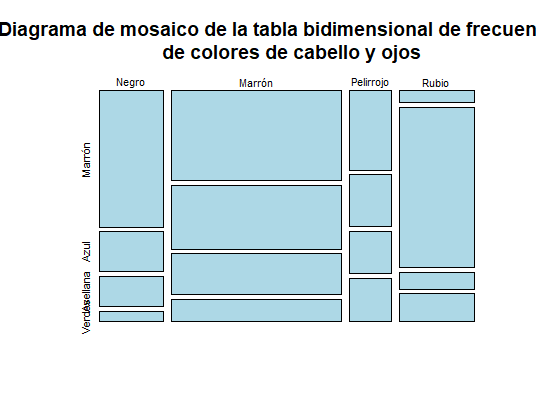
\includegraphics[scale=0.7]{Mosaico}
\caption{Representación grafica de mosaico}
\label{fig:Mosaico}
\end{figure}

\newpage


\subsection{Estadística descripitiva de una variable}

En las sigientes gáficas se muestra la variación que hay entre el color de cabello \ref{f:DensityCabello}, color de ojos   \ref{f:DensityOjos} y el género mayor volube en cuanto a distincion del color de ojos y cabello\ref{f:DensitySexo}, ya que estas son una variación. 


\begin{figure}[h]
 \centering
  \subfloat[Cabello]{
   \label{f:DensityCabello}
    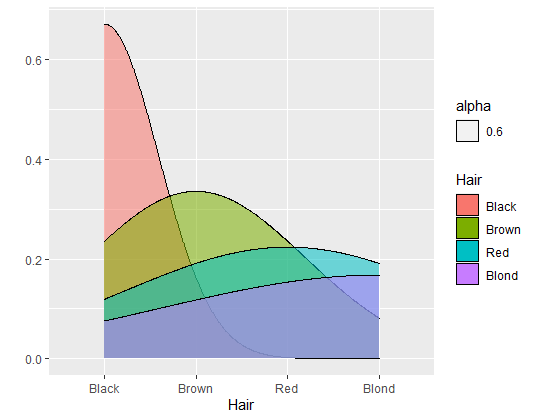
\includegraphics[width=0.3\textwidth]{DensityCabello}}
  \subfloat[Ojos]{
   \label{f:DensityOjos}
    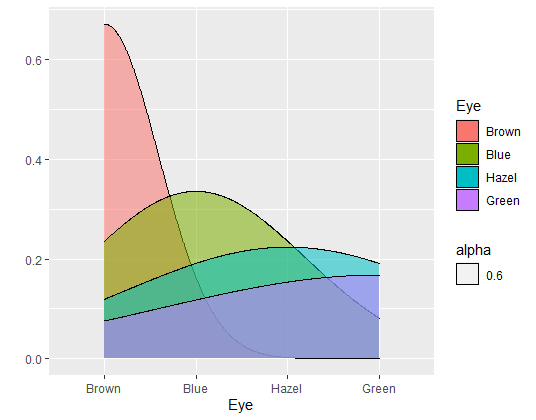
\includegraphics[width=0.3\textwidth]{DensityOjos}}
  \subfloat[Sexo]{
   \label{f:DensitySexo}
    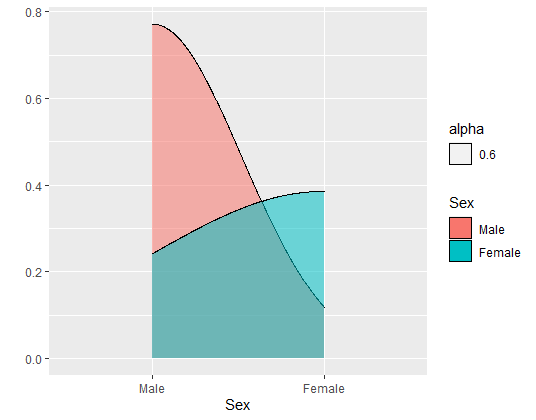
\includegraphics[width=0.3\textwidth]{DensitySexo}}
 \caption{Density plot de cabello, ojos y sexo}
 \label{f:Density}
\end{figure}


\begin{figure}[ht]
 \centering
  \subfloat[Ojos]{
   \label{f:FrecuenciaOjos}
    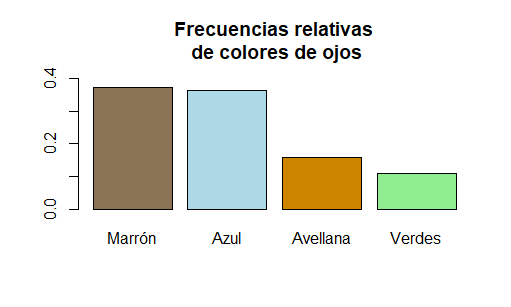
\includegraphics[width=0.4\textwidth]{FrecuenciaOjos}}
  \subfloat[Cabello]{
   \label{f:FrecuenciaCabello}
    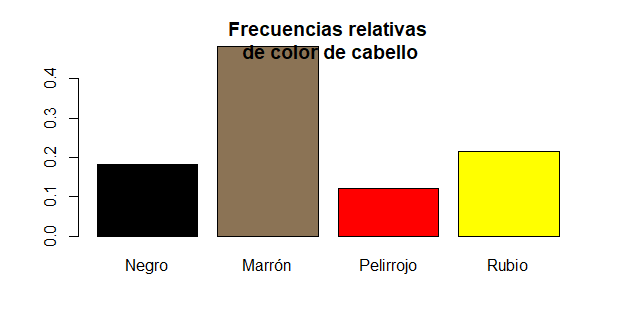
\includegraphics[width=0.4\textwidth]{FrecuenciaCabello}}
 \caption{Frecuencia de color de cabello y de ojos}
 \label{f:Frecuencias}
\end{figure}

\newpage

\begin{figure}
 \centering
  \subfloat[Ojos]{
   \label{f:FrecuenciaOjosCabello}
    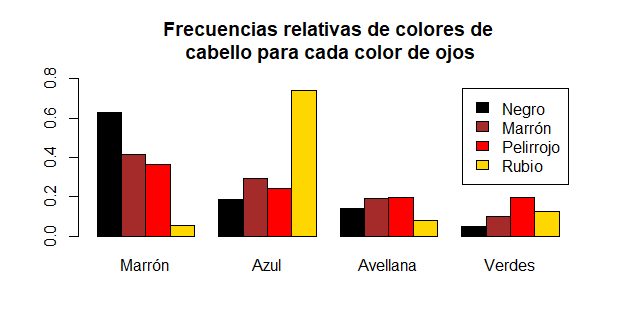
\includegraphics[width=0.4\textwidth]{FrecuenciaOjosCabello}}
  \subfloat[Cabello]{
   \label{f:FrecuenciaCabelloOjos}
    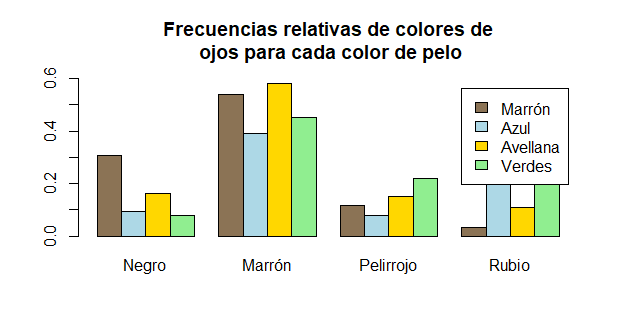
\includegraphics[width=0.4\textwidth]{FrecuenciaCabelloOjos}}
 \caption{Frecuencia correlativa entre el color de cabello y de ojos}
 \label{f:Frecuencias2}
\end{figure}

\newpage
\subsection{Estadística descripitiva de dos variable}

\begin{figure}
 \centering
  \subfloat[Sexo]{
   \label{f:Box1}
    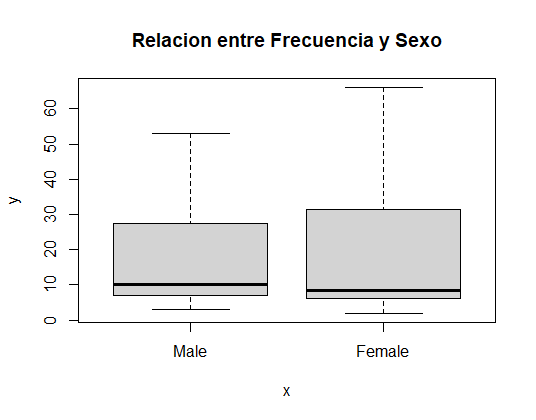
\includegraphics[width=0.3\textwidth]{Box1}}
  \subfloat[Cabello]{
   \label{f:BoxCabello}
    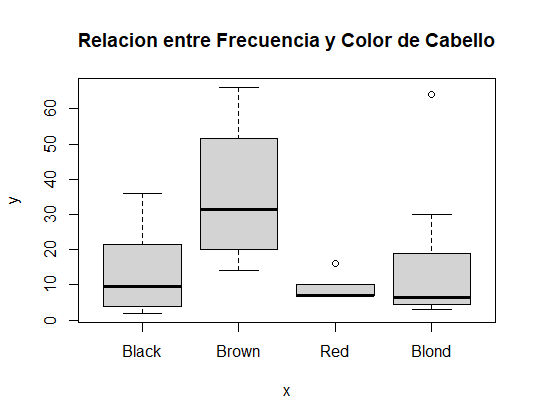
\includegraphics[width=0.3\textwidth]{BoxCabello}}
  \subfloat[Ojos]{
   \label{f:BoxOjos}
    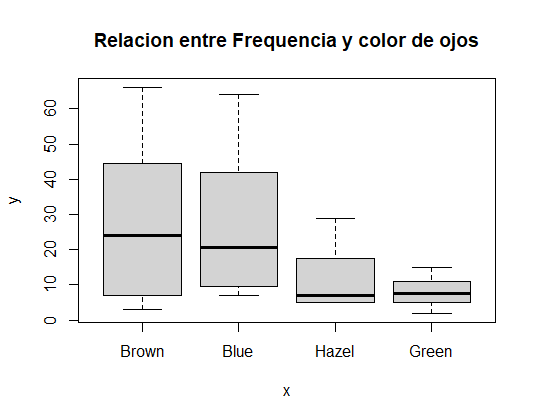
\includegraphics[width=0.3\textwidth]{BoxOjos}}
 \caption{Box de correlación entre frecuencia y las variables}
 \label{f:Box}
\end{figure}

\begin{figure}
 \centering
  \subfloat[Cabello]{
   \label{f:BoxplotCabello}
    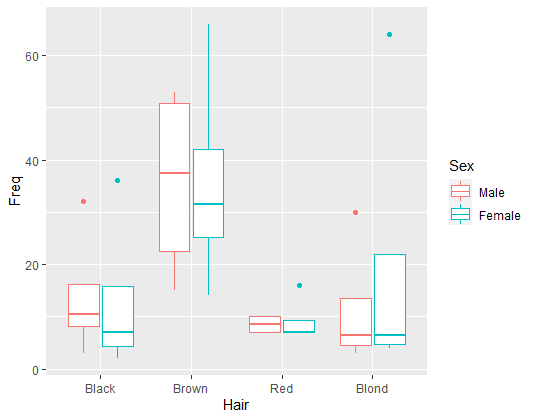
\includegraphics[width=0.4\textwidth]{BoxplotCabello}}
  \subfloat[Ojos]{
   \label{f:BoxplotOjos}
    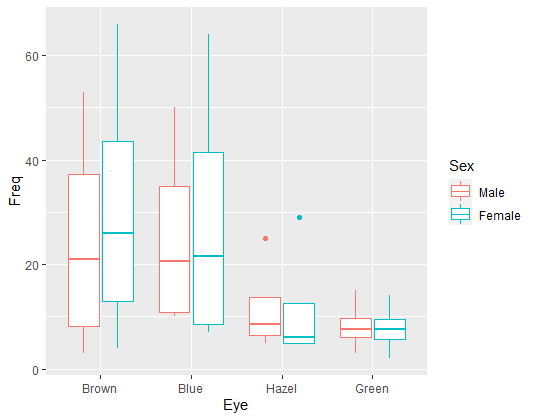
\includegraphics[width=0.4\textwidth]{BoxplotOjos}}
 \caption{Boxplot de correlación entre género y color de cabello y ojos}
 \label{f:Boxplot}
\end{figure}


\begin{figure}
\centering
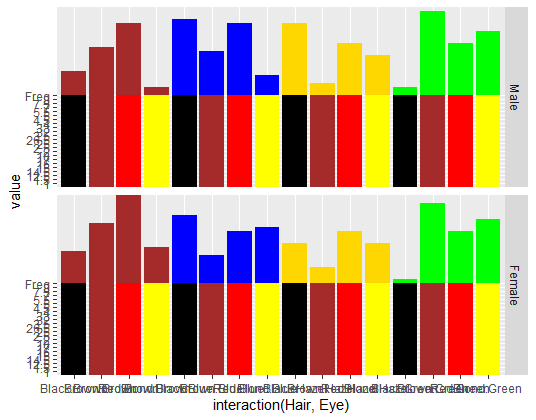
\includegraphics[scale=0.8]{Escala}
\caption{Escala de variación}
\label{fig:Escala}
\end{figure}

\newpage
\section{Conclusión}


\newpage

\section{Referencias}

Cynthia Ivanna Cruz Quiñones\citep{repositorio}

\bibliography{biblio}
\bibliographystyle{plainnat}


\end{document}



\end{document}
